%%%%%%%%%%%%%%%%%%
% General config %
%%%%%%%%%%%%%%%%%%

\documentclass{article}
\usepackage[margin=1.2in]{geometry}
\usepackage[english]{babel}

%%%%%%%%%%%%
% Packages %
%%%%%%%%%%%%

% Math packages
\usepackage{amsthm}
\usepackage{amsmath,amssymb}
\usepackage{amsfonts,mathtools}
% \usepackage{thmbox}
\usepackage{bm}
\usepackage{proof-at-the-end}

% graphics packages
\usepackage{pict2e,picture}
\usepackage{graphicx}
\usepackage{tikz}
\usetikzlibrary {positioning,graphs,calc,decorations.pathmorphing,shapes,arrows.meta,arrows,shapes.misc}
\usetikzlibrary{topaths,calc}
\usetikzlibrary{fit}
\usepackage{subcaption}
\usepackage{xcolor}
\usepackage{wrapfig}
\usepackage{float}

% custom environments
\usepackage{comment}
\usepackage{enumitem}
\usepackage{epigraph}
\usepackage{environ}
\usepackage{listings}

% Miscellanious packages
\usepackage{lipsum,mwe,abstract}
\usepackage{multicol}
\usepackage{refcount}
\usepackage{hyperref}
\usepackage{censor}
\usepackage[numbers]{natbib}



%%%%%%%%%%%%%%%%%%%
% Custom Commands %
%%%%%%%%%%%%%%%%%%%

% covering relation
\newcommand{\coveringA}{%
  \mathrel{-\mkern-4mu}<%
}
\newcommand{\coveringB}{\mathrel{\text{$\vcenter{\hbox{\pictcoveringB}}$}}}
\newcommand{\pictcoveringB}{%
  \begin{picture}(1em,.5em)
    \roundcap
    \put(0,.25em){\line(1,0){.6em}}
    \put(.6em,.25em){\line(3,1){.4em}}
    \put(.6em,.25em){\line(3,-1){.4em}}
  \end{picture}%
}

% highlight
\newcommand{\highlight}[1]{%
  \par\noindent
  \colorbox{gray!30}{%
    \parbox{\dimexpr\linewidth-2\fboxsep\relax}{%
      #1
    }%
  }}

% custom theorem environments
\theoremstyle{plain}
\newtheorem{theorem}{Theorem}[section]
\newtheorem{corollary}[theorem]{Corollary}
\newtheorem{lemma}[theorem]{Lemma}
\newtheorem{prop}[theorem]{Proposition}

\theoremstyle{definition}
\newtheorem{definition}[theorem]{Definition}
\newtheorem{example}[theorem]{Example}
\newtheorem{property}[theorem]{Property}
\newtheorem{notation}[theorem]{Notation}
\newtheorem{convention}[theorem]{Convention}
\newtheorem{interpretation}[theorem]{Interpretation}
\newtheorem{remark}[theorem]{Remark}
% \newtheorem{question}[theorem]{Question}
\newtheorem{note}[theorem]{Note}

\newtheorem{question}{Question}
\theoremstyle{plain}
\newtheorem{assertion}{Assertion}[question]

\newenvironment{reponse}{\renewcommand{\proofname}{Réponse}\begin{proof}}{\end{proof}}

% special theorems / definitions / lemmas
\newtheoremstyle{specialthm}% name
{\topsep}%   Space above
{\topsep}%   Space below
{\itshape}%  Body font
{}%          Indent amount
{\bfseries}% Theorem head font
{}%          Punctuation after theorem head -- blank
{0.5em}%     Space after theorem head (0.5em is the default)
{{\thmname{#1}\thmnumber{ #2$^{\bm*}\!$}\thmnote{\ \textmd{(#3)}.}}}

\theoremstyle{specialthm}
\newtheorem{sptheorem}[theorem]{Theorem}
\newtheorem{spcorollary}[theorem]{Corollary}
\newtheorem{splemma}[theorem]{Lemma}
\newtheorem{spprop}[theorem]{Proposition}

% special theorems / definitions / lemmas
\newtheoremstyle{specialdef}% name
{\topsep}%   Space above
{\topsep}%   Space below
{}%  Body font
{}%          Indent amount
{\bfseries}% Theorem head font
{}%          Punctuation after theorem head -- blank
{0.5em}%     Space after theorem head (0.5em is the default)
{{\thmname{#1}\thmnumber{ #2$^{\bm*}\!$}\thmnote{\ \textmd{(#3)}.}}}

\theoremstyle{specialdef}
\newtheorem{spdefinition}[theorem]{Definition}
\newtheorem{spproperty}[theorem]{Property}

% abstract customization
\renewenvironment{abstract}
{\small
  \begin{center}
    \bfseries \abstractname\vspace{-.5em}\vspace{0pt}
  \end{center}
  \list{}{
    \setlength{\leftmargin}{20mm}
    \setlength{\rightmargin}{\leftmargin}
  }
\item\relax}
{\endlist}

% special epigraph/acknowledgements
\newenvironment{dedication}
{\clearpage           % we want a new page
  \vspace*{\stretch{1}}% some space at the top
  \itshape             % the text is in italics
  \raggedleft          % flush to the right margin
  \begin{minipage}{0.6\linewidth}
    \parindent=12pt
  }
  {\end{minipage}
  \par % end the paragraph
  \vspace{\stretch{2}} % space at bottom is three times that at the top
  \raggedleft
  \textit{All Finite Lattices are Algebraic Lattices.}\\
  \textit{-- G. Birkhoff}
  \vspace{\stretch{1}}
  \clearpage           % finish off the page
}

% Size for partition
% \def\Bign#1{\mathclose{\hbox{$\left#1\vbox to11.5\p@{}\right.\n@space$}}\mathopen{}}

% equiv class
\def\equivclass{/}

\title{\Large Ordered sets}
\date{06/16/21}

\begin{document}

\maketitle

% --------------- ABSTRACT
\begin{abstract}
  Definitions and examples about ordered sets. Followed the first chapter of
  Davey and Priestley's Introduction to Lattices and Order (2002)
\end{abstract}

\docrule

% --------------- MAIN CONTENT

\section{Introduction to Ordered sets}

\begin{definition}
	Let $P$ be a set. An \textbf{order} (or \textbf{partial order}) on $P$ is a binary relation $\leq$ such that $\forall x,y,z \in P$:
	\begin{enumerate}
		\item $x \leq x$ (Reflexivity)
		\item $x \leq y$ and $y \leq x$ implies $x=y$ (Antisymmetry)
		\item $x \leq y$ and $y \leq z$ implies $x \leq z$ (Transitivity)
	\end{enumerate}
\end{definition}

\begin{remark}
	A set $P$ equiped with an order relation is said to be a poset (partialy ordered set)
\end{remark}

\begin{definition}[Order-isomorphism]\label{def:order-isomorphism}
	Let $P$ and $Q$ be two ordered sets. We say that $P$ and $Q$ are \textbf{order-isomorphic} (or just \textbf{isomorphic}) and write $P \cong Q$ if there exists a map $\varphi$ from $P$ onto $Q$ such that $x \leq y$ in $P$ iff $\varphi(x) \leq \varphi(y)$ in $Q$. Then $\varphi$ is called an \textbf{order isomorphism}.
\end{definition}

\begin{remark}
	$\varphi$ is neccessarly bijective but in the other hand not every bijective map between ordered sets is an order-isomorphism.
\end{remark}

\begin{definition}[Covering relation]
	Let $P$ be an ordered set and let $x,y \in P$. We say $x$ is \textbf{covered by} $y$ (or $y$ \textbf{covers} $x$) and write $x \coveringB y$. If $x < y$ and $x \leq z < y$, then $x = z$.

	The latter condition is demanding that there be no element $z$ of $P$ with $x < z < y$ if $x \coveringB y$.
\end{definition}

\begin{remark}
	Here $<$ is defined by: $x < y$ iff $x \leq y$ and $x \neq y$.
\end{remark}

\begin{remark}
	We understand the covering relation as indicating that if $x \coveringB y$, there exists no element between them (if such an element would exist, it would have to be $x$)
\end{remark}

\begin{example}
    Let's consider the natural numbers $\mathbb{N}$. We have $m \coveringB n$ iff $n = m+1$: this means that no other element exists between two successive natural numbers.
\end{example}

\begin{definition}[Hasse Diagram]
	Let $P$ be a finite ordered set. We can represent $P$ by a configuration of circles (elements of $P$) and interconnecting lines (indicating the covering relation). We can construct it as follows:
    \begin{enumerate}
    \item To each point $x \in P$, associate a point $p(x)$ of the Euclidian plane depicted by a small circle.
    \item For each covering pair $x \coveringB y$ in $P$, take a line segment $l(x,y)$ joining the circle at $p(x)$ to the circle at $p(y)$
    \item Carry out (1) and (2) in such a way that
          \begin{enumerate}
          \item if $x \coveringB y$ then $p(x)$ is lower than $p(y)$ ($p(y)$ is represented above $p(x)$)
          \item the circle at $p(z)$ does not intersect the line segment $l(x,y)$ if $z \neq x$ and $z \neq y$
          \end{enumerate}
    \end{enumerate}
\end{definition}

\begin{example}
Let's consider the ordered set $P = \{a,b,c,d\}$ in which $a<c, a<d, b<c, b<d$.

Here is an example of a valid Hasse diagram:

\begin{center}
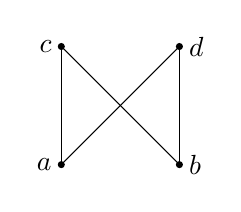
\begin{tikzpicture}[scale=.75]
\draw[fill] (-1, 0) circle (.05cm) node[left] {$a$};
\draw[fill] (1, 0) circle (.05cm) node[right] {$b$};
\draw[fill] (-1, 2) circle (.05cm) node[left] {$c$};
\draw[fill] (1, 2) circle (.05cm) node[right] {$d$};
\draw (-1,0) -- (1,2);
\draw (-1,0) -- (-1,2);
\draw (1,0) -- (-1,2);
\draw (1,0) -- (1,2);
\end{tikzpicture}
\end{center}

There is a problem with the following one: we have $a <c$, so $a$ should be lower than $c$. We can never have two connected nodes at the same height. If there is a covering, one must be lower than the other.

\begin{center}
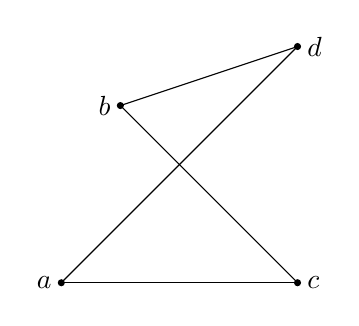
\begin{tikzpicture}[scale=.75]
\draw[fill] (-1,1) circle (.05cm) node[left] {$b$};
\draw[fill] (2, 2) circle (.05cm) node[right] {$d$};
\draw[fill] (2, -2) circle (.05cm) node[right] {$c$};
\draw[fill] (-2, -2) circle (.05cm) node[left] {$a$};
\draw (-1,1) -- (2,2);
\draw (-1,1) -- (2,-2);
\draw (-2,-2) -- (2,-2);
\draw (-2,-2) -- (2,2);
\end{tikzpicture}
\end{center}

We should also avoid confusing node placements: even if the relations are well defined in tikz, when we look at the resulting diagram we can't see if $a$ and $c$ are connected - and we may think that $c$ and $d$ are.

\begin{center}
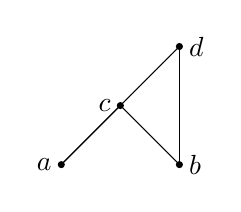
\begin{tikzpicture}[scale=.75]
\draw[fill] (-1, 0) circle (.05cm) node[left] {$a$};
\draw[fill] (1, 0) circle (.05cm) node[right] {$b$};
\draw[fill] (0, 1) circle (.05cm) node[left] {$c$};
\draw[fill] (1, 2) circle (.05cm) node[right] {$d$};
\draw (-1,0) -- (1,2);
\draw (-1,0) -- (0,1);
\draw (1,0) -- (0,1);
\draw (1,0) -- (1,2);
\end{tikzpicture}
\end{center}

\end{example}

\begin{prop}
Two finite ordered sets $P$ and $Q$ are \textbf{order-isomorphic} iff they can be drawn with identical diagrams.
\end{prop}

\section{Constructing and de-constructing ordered sets}

\begin{definition}[Dual set]
Given any ordered set $P$ we can form a new ordered set $P^{\partial}$ (the \textbf{dual} of $P$) by defining $x \leq y$ to hold in $P^{\partial}$ iff $y \leq x$ holds in $P$.
\end{definition}

\begin{remark}
For $P$ finite we obtain a diagram for $P^{\partial}$ by ``turning upside down'' the Hasse diagram for $P$.
\end{remark}

\begin{definition}[bottom / top]
	Let $P$ be an ordered set, we say $P$ as a \textbf{bottom} element if there exists $\bot \in P$ with the proprety that $\forall x \in P, \bot \leq x$. Dually, $P$ as a \textbf{top} element if there exists $\top \in P$ such that $\forall x \in P, x \leq \top$.
\end{definition}

\begin{definition}[lifting]
	Given an ordered set $P$ (with or without $\bot$) we form $P_{\bot}$ (called \textbf{$P$ lifted}) as follows: take an element $0 \not \in P$ and define $\leq$ on $P_{\bot} := P \cup\{0\}$ by:

	\begin{equation*}
		x \leq y \text{ if and only if } x = 0 \text{ or } x \leq y \text{ in } P
	\end{equation*}
\end{definition}

\begin{remark}
	We will see that lifting is usefull for transforming ordered sets into lattices.
\end{remark}

\begin{question}
	Antichain $\bar S$: it seems to be used to define sums of ordered sets.
\end{question}

\begin{definition}[disjoint union]
  Suppose that $P$ and $Q$ are disjoint ordered sets. The \textbf{disjoint union} $P \cup U$ of $P$ and $Q$ is the ordered set formed by defining $x \leq y$ in $P \cup Q$ if and only if either $x, y \in P$ and $x \leq y$ in $P$ or $x,y \in Q$ and $x \leq y$ in $Q$.
\end{definition}

\begin{remark}
  A diagram for $P \cup Q$ is formed by placing diagrams for $P$ and $Q$ side by side.
\end{remark}

\begin{definition}[sums of ordered sets]
	The \textbf{linear sum} of two disjoint ordered sets $P$ and $Q$ ($P \oplus Q$) is defined by taking the following order relation on $P \cup Q: x \leq y$ if and only if:
	\begin{align*}
		& x,y \in P \text{ and } x \leq y \text{ in } P, \\
		\text{ or } & x,y \in Q \text{ and } x \leq y \text{ in } Q, \\
		\text{ or } & x \in P \text{ and } y \in Q
	\end{align*}

	A diagram for $P \oplus Q$ (when $P,Q$ finite) is obtained by placing a diagram for $P$ directly below a diagram for $Q$ and then adding a line segment from each maximal element of $P$ to each minimal element of $Q$.
\end{definition}

\begin{remark}
	The lifting construction is a special case of a linear sum: $P_{\bot}$ is just $1 \oplus P$. Similarly, $P \oplus 1$ represents $P$ with a top element added.
\end{remark}

\begin{prop}
	Each of the operation $\cup$ and $\oplus$ is associative.
\end{prop}

\begin{definition}[antichain]
  Let $P$ be an ordered set, and $S$ a non-empty subset of $P$. The \textbf{antichain} $\bar S$ is the set of all elements in $S$ such that no two of which are comparable with each other.n
\end{definition}

\begin{interpretation}
Intuitively, an antichain $\bar S$ of a subset $S$ of $P$ is $S$ but without any of the covering relations: that is, all elements of $\bar S$ are non-comparable.
\end{interpretation}

\begin{remark}
  As such, the elements in a representation of an antichain are always alligned.
\end{remark}

\begin{remark}
  We have $\bar 1 = 1$
\end{remark}

\begin{notation}
  We can denote by $n$, $n$ being a natural number, a chain of $n$ pair-wise connected elements. We can also define as $\bar n$ an antichain of size $n$.
  \begin{example}
    Here we define a poset as $3$ and an antichain as $\bar 3$.

    \begin{figure}
      \centering
      \begin{subfigure}{0.5\textwidth}
        \centering
        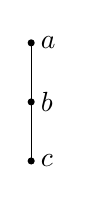
\begin{tikzpicture}[scale=.75]
          \draw[fill] (0, 2) circle (.05cm) node[right] {$a$};
          \draw[fill] (0, 1) circle (.05cm) node[right] {$b$};
          \draw[fill] (0, 0) circle (.05cm) node[right] {$c$};
          \draw (0,0) -- (0,1);
          \draw (0,1) -- (0,2);
        \end{tikzpicture}
        \caption*{3}
      \end{subfigure}%
      \begin{subfigure}{0.5\textwidth}
        \centering
        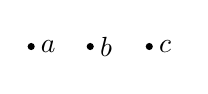
\begin{tikzpicture}[scale=.75]
          \draw[fill] (0, 0) circle (.05cm) node[right] {$a$};
          \draw[fill] (1, 0) circle (.05cm) node[right] {$b$};
          \draw[fill] (2, 0) circle (.05cm) node[right] {$c$};
        \end{tikzpicture}
        \caption*{$\bar 3$}
      \end{subfigure}
    \end{figure}
  \end{example}
\end{notation}

\begin{definition}[$M_n$]
  We define a class of ordered sets $M_n$, with $n \in \mathbb{N}^*$, as $M_n = 1 \oplus \bar n \oplus 1$
\end{definition}

\begin{example}
  Here are several examples of ordered sets constructed via sums and disjoint unions.
  \begin{center}
    \includegraphics[width = 0.6\textwidth]{images/sums.png}
  \end{center}

  The diagram of $\bar 1 \oplus \bar 2 \oplus \bar 3$ is constructed by placing the antichain of $1$, $2$ and $3$ from the botom to the top ordered from left to right in the equation. Then, we connect the minimal elements to the maximum elements between groups (except for the extremi groups).
  To construct $M_2 \oplus M_3$ we follow the same rules. The construction of $M_n$ (here $n=2$ and $n=3$) is as follows: we draw an antichain of size $n$ as well as a top and botom element which we then connect to each element of the antichain.

   \begin{remark}
	   We do not 'merge' elements when doing an ordered sets summation: the botom and top elements of $M_2$ and $M_3$ are two disctinct elements edged to each other. Therefore, the cardinaltity of set summation should always be equal to the sum of the cardinals of each groups.
   \end{remark}

  The ordered set $2 \oplus 3 \cong 5$ means that the direct sum of $2$ and $3$ is order-isomorphic to $5$.
\end{example}



\begin{definition}[down-set / up-set]
Let $P$ be an ordered set and $Q \subseteq P$.
\begin{enumerate}
\item $Q$ is a \textbf{down-set} if, whenever $x \in Q$, $y \in P$ and $y \leq x$, we have $y \in Q$.
\item Dually, $Q$ is an \textbf{up-set} if, whenever $x \in Q$, $y \in P$ and $x \leq y$ we have $y \in Q$.
\end{enumerate}
\end{definition}

\begin{example}
Let $P$ be an ordered set, with the following Hasse diagram:
\begin{center}
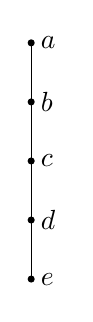
\begin{tikzpicture}[scale=.75]
\draw[fill] (0, 3) circle (.05cm) node[right] {$a$};
\draw[fill] (0, 2) circle (.05cm) node[right] {$b$};
\draw[fill] (0, 1) circle (.05cm) node[right] {$c$};
\draw[fill] (0, 0) circle (.05cm) node[right] {$d$};
\draw[fill] (0, -1) circle (.05cm) node [right] {$e$};
\draw (0,3) -- (0,2);
\draw (0,2) -- (0,1);
\draw (0,1) -- (0,0);
\draw (0,0) -- (0,-1);
\end{tikzpicture}
\end{center}

Here, $S = \{d,e\}$ is a down-set of $P$: for $x \in S$, there is no element $y \in P$ such that $y \leq x$ if $y \notin S$.

The preceding example is a bit simple: let's do it with a set with more branching.

\begin{center}
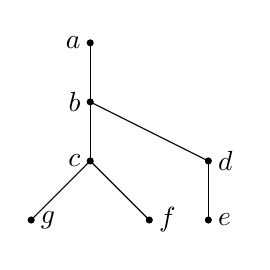
\begin{tikzpicture}[scale=.75]
\draw[fill] (0, 3) circle (.05cm) node[left] {$a$};
\draw[fill] (0, 2) circle (.05cm) node[left] {$b$};
\draw[fill] (0, 1) circle (.05cm) node[left] {$c$};
\draw[fill] (2, 1) circle (.05cm) node[right] {$d$};
\draw[fill] (2, 0) circle (.05cm) node[right] {$e$};
\draw[fill] (1, 0) circle (.05cm) node[right] {$f$};
\draw[fill] (-1,0) circle (.05cm) node[right] {$g$};
\draw (0,3) -- (0,2);
\draw (0,2) -- (0,1);
\draw (0,2) -- (2,1);
\draw (2,1) -- (2,0);
\draw (0,1) -- (1,0);
\draw (0,1) -- (-1,0);
\end{tikzpicture}
\end{center}

Here we can define two independent down-sets: $\{g,c,f\}$ and $\{d,e\}$ (which wasn't the case with the previous example - all of the downsets share the same lowest element). But yet, we can't define two indepentent up-sets (all up-sets would share $a$ as a top element).
\end{example}


\begin{definition}[down/up of a subset]
Given an arbitrary subset $S$ of $P$ we can define $\downarrow S$ and $\uparrow S$, which are read ``down S'' and ``up S'' respectively:
\begin{equation*}
\downarrow S := \{ y \in P | \exists x \in S, y \leq x \} \text{ and } \uparrow S := \{ y \in P | \exists x \in S, x \leq y \}
\end{equation*}
\end{definition}

\begin{remark}
$\downarrow S$ is the smallest down-set containing $S$. Respectively for $\uparrow S$, which is the smallest up-set containing $S$.

$S$ is a down-set (up-set) iff $S = \downarrow S$ ($S = \uparrow S$).
\end{remark}

\begin{definition}[down/up of an element]
Given an element $x \in P$, we define $\downarrow x$ and $\uparrow x$:

\begin{equation*}
\downarrow x := \{ y \in P | y \leq x \} \text{ and } \uparrow x := \{ y \in P | x \leq y \}
\end{equation*}
\end{definition}

\begin{remark}
This is a special case of the previous definition, given a unit set.
\end{remark}

\begin{notation}
  The family of all down-sets of $P$ is denoted by $\mathcal{O}(P)$
\end{notation}

\begin{lemma}
  Let $P$ be an ordered set. $\forall Q \in \mathcal{O}(P)$, $x \in Q \iff \downarrow x \subseteq Q$.
\end{lemma}

\begin{proof}
  Let $Q \in \mathcal{O}(P)$

  We have $x \in \downarrow x$. As such, $\downarrow x \subseteq Q \implies x \in Q$.

  Now, let's suppose $x \in Q$. By definition, $\downarrow x = \{y \in P | y \leq x\}$. We know that whenever $x \in Q$, $\forall a \in P$ such that $a \leq x$, $a \in Q$. Given that $\forall a \in \downarrow x$, $a \leq x$, we have $a \in Q$. So, $\downarrow x \subseteq Q$.
\end{proof}

\begin{lemma}
  Let $P$ be an ordered set and $x,y \in P$. Then the following are equivalent:
  \begin{itemize}
  \item $x \leq  y$
  \item $\downarrow x \subseteq \downarrow y$
  \item $\forall Q \in \mathcal{O}(P)$, $y \in Q \implies x \in Q$
  \end{itemize}
\end{lemma}

\begin{proof}
	\underline{i. $\rightarrow$ ii.} Suppose $x \leq y$ and let $a \in \downarrow x$; then $a \leq x$ so by transitivity $a \leq y$, meaning $a \in \downarrow y$.

\

\underline{ii. $\rightarrow$ iii.} Suppose $\downarrow x \subseteq \downarrow y$. We want to prove that for any $Q$ in $\mathcal{O}(P)$, $y \in Q \Rightarrow x \in Q$. Which, by the previous lemma, is equivalent to proving that $\downarrow x \subseteq Q \Rightarrow \downarrow y \subseteq Q$. If $\downarrow x \subseteq Q$, and given that we supposed $\downarrow x \subseteq \downarrow y$, then it is clear that $\downarrow y \subseteq Q$ (by transitivity).

\

\underline{iii. $\rightarrow$ i.} Suppose $\forall Q \in \mathcal{O}(P), y \in Q \Rightarrow x \in Q$. Now we suppose that $y < x$. We can choose $Q = \downarrow y \in \mathcal{O}(P)$ (the smallest down-set containing $y$), since the first hypothesis must be valid for all downsets of $P$. But, since $x \notin  Q$, by our previous assumption - we have a direct contradiction to our first hypothesis: by reductio ad absurdum, $x \leq y$.

We have now proven the previous lemma by circularity.
\end{proof}

\begin{lemma}
    $Q$ is a down-set of $P$ if and only if $P \setminus Q$ is an up-set of $P$.
\end{lemma}

\begin{proof}
  Let $Q \in \mathcal{O}(P)$ such that $Q$ is non-empty. We can choose $x \in Q$ such that $Q = \downarrow x$ (so $x \in \text{Max } Q$).

  Let's prove that $P \setminus Q = \uparrow x$


\end{proof}

\begin{lemma}
  For subsets $A,B \in P$, we have $A \subseteq B$ if and only if $P \setminus B \subseteq P \setminus A$.
\end{lemma}

\begin{proof}

\end{proof}

\begin{prop}
  $\mathcal{O}(P)^{\partial} \cong \mathcal{O}(P^{\partial})$.
\end{prop}

\begin{proof}

\end{proof}

\begin{definition}
Let $P$ and $Q$ be ordered sets. A map $\varphi: P \rightarrow Q$ is said to be:
\begin{enumerate}
\item \textbf{order-preserving}(also called \textbf{monotone}) if $x \leq y$ in $P$  implies $\varphi(x) \leq \varphi(y)$ in $Q$
\item an \textbf{order-embedding} if $x \leq y$ in $P$ if and only if $\varphi(x) \leq \varphi(y)$ in $Q$
\item an \textbf{order-isomorphism} if it is an order-embedding which maps $P$ onto $Q$ (refer to definition 1.2)
\end{enumerate}
\end{definition}

\begin{remark}
It is worth noting that an order-embedding is not necessarily bijective, unlike an order-isomorphism.
\end{remark}

\begin{example}
	Consider the following maps between ordered sets.
	\begin{center}
		\includegraphics[scale = 0.5]{./images/mapping.png}
	\end{center}

	We can show that:
	\begin{itemize}
		\item $\phi_1$ is not order-preserving.
		\item Each of $\phi_2$ to $\phi_5$ is order-preserving but not an order-embedding.
		\item The map $\phi_6$ is an order-embedding but not an order-isomorphism.
	\end{itemize}

	\

	In order for $\phi_1$ to be order-preserving it would need to satisfy, for any $a,b: a \leq b \Rightarrow \phi_1(a) \leq \phi_1(b)$. Yet, for instance, $a \leq d$ implies $\phi_1(d) \leq \phi_1(a)$ and $a \neq d$ (we could also look at $a$ and $b$ to prove that it is not order-preserving).

	\

	On the other hand, $\phi_2$ is order-preserving. We can check element by element:
	\begin{enumerate}
		\item $d \leq e$ and $\phi_2(d) \leq \phi_2(e)$.
		\item $b \leq d$ and $\phi_2(b) \leq \phi_2(d)$.
		\item $c \leq d$ and $\phi_2(c) = \phi_2(d)$ so $\phi_2(c) \leq \phi_2(d)$.
		\item $a \leq b$ and $\phi_2(a) = \phi_2(b)$ so $\phi_2(a) \leq \phi_2(b)$.
		\item $a \leq c$ and $\phi_2(a) \leq \phi_2(c)$.
	\end{enumerate}
	Yet, $\phi_2$ is not an order embedding. For instance, $\phi_2(a) = \phi_2(b) \not \Rightarrow a \leq b$.

	\

	In the six examples, only $\phi_6$ is an order-embedding. All relations $b \leq d$, $c \leq d$, $a \leq b$ and $a \leq c$ are present after $\phi_6$ was applied. Still, $\phi_6$ is not an order-isomorphism as elements in the order-set resulting from $\phi_6$ do not exist in the original set (not bijective).

\end{example}

\begin{definition}[products]
	Let $P_1, ..., P_n$ be ordered sets. The Cartesian product $P_1 \times ... \times P_n$ can be made into an ordered set by imposing the coordinatewise order defined by:

	$$(x_1, ..., x_n) \leq (y_1, ..., y_n) \Leftrightarrow (\forall i) x_i \leq y_i \text{ in } P_i$$
\end{definition}

\begin{remark}
	Intuitively, a product $P \times Q$ is drawn by replacing each point of a diagram of $P$ by a copy of a diagram for $Q$, and connecting 'corresponding' points; this assumes that the points are placed in such a way that the rules for diagram drawing in definition 1.4 are obeyed.
\end{remark}


\begin{example}
  We can construct the following poset by combining


\begin{figure}[h!]
  \centering
  \begin{subfigure}{0.266\textwidth}
    \centering
    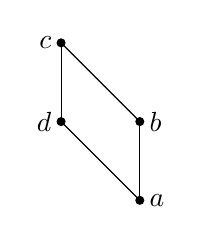
\begin{tikzpicture}
      \draw[fill] (0,-1) circle (.05cm) node[right] {$a$};
      \draw[fill] (0,0) circle (.05cm) node[right] {$b$};
      \draw[fill] (-1,1) circle (.05cm) node[left] {$c$};
      \draw[fill] (-1,0) circle (.05cm) node[left] {$d$};

      \draw (0,-1) -- (0,0);
      \draw (0,0) -- (-1,1);
      \draw (-1,1) -- (-1,0);
      \draw (-1,0) -- (0,-1);

    \end{tikzpicture}
    \caption*{$M_2$}
  \end{subfigure}%
  \begin{subfigure}{0.1\textwidth}
    \centering
    $\times$
  \end{subfigure}%
  \begin{subfigure}{0.266\textwidth}
    \centering
    \begin{tikzpicture}
      \draw[fill] (0,-1) circle (.05cm) node[right] {$1$};
      \draw[fill] (1,0) circle (.05cm) node[right] {$2$};
      \draw[fill] (2,1) circle (.05cm) node[right] {$3$};

      \draw (0,-1) -- (2,1);
      \draw (2,1) -- (1,0);
      \draw (1,0) -- (0,-1);
    \end{tikzpicture}
    \caption*{3}
  \end{subfigure}%
  \begin{subfigure}{0.1\textwidth}
    \centering
    $=$
  \end{subfigure}%
    \begin{subfigure}{0.266\textwidth}
      \centering
      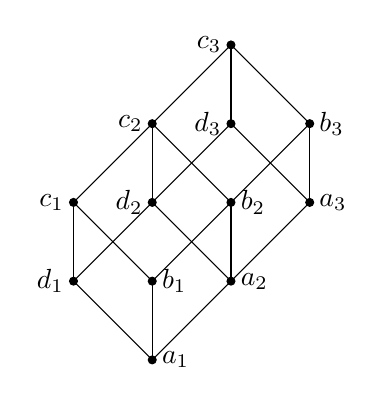
\begin{tikzpicture}

      \draw[fill] (0,-1) circle (.05cm) node[right] {$a_1$};
      \draw[fill] (0,0) circle (.05cm) node[right] {$b_1$};
      \draw[fill] (-1,1) circle (.05cm) node[left] {$c_1$};
      \draw[fill] (-1,0) circle (.05cm) node[left] {$d_1$};

      \draw[fill] (1,0) circle (.05cm) node[right] {$a_2$};
      \draw[fill] (1,1) circle (.05cm) node[right] {$b_2$};
      \draw[fill] (0,2) circle (.05cm) node[left] {$c_2$};
      \draw[fill] (0,1) circle (.05cm) node[left] {$d_2$};

      \draw[fill] (2,1) circle (.05cm) node[right] {$a_3$};
      \draw[fill] (2,2) circle (.05cm) node[right] {$b_3$};
      \draw[fill] (1,3) circle (.05cm) node[left] {$c_3$};
      \draw[fill] (1,2) circle (.05cm) node[left] {$d_3$};

      \draw (0,2) -- (-1,1);
      \draw (0,2) -- (1,1);
      \draw (0,2) -- (0,1);
      \draw (0,1) -- (-1,0);
      \draw (0,1) -- (1,0);
      \draw (1,0) -- (0,-1);
      \draw (-1,0) -- (0,-1);
      \draw (-1,1) -- (0,0);
      \draw (1,1) -- (0,0);
      \draw (0,0) -- (0,-1);
      \draw (-1,1) -- (-1,0);
      \draw (1,1) -- (1,0);

      \draw (2,1) -- (2,2);
      \draw (2,2) -- (1,3);
      \draw (1,3) -- (1,2);
      \draw (1,2) -- (2,1);

      \draw (1,0) -- (2,1);
      \draw (1,1) -- (2,2);
      \draw (0,2) -- (1,3);
      \draw (0,1) -- (1,2);
    \end{tikzpicture}
    \caption*{$M_2 \times 3$}
  \end{subfigure}
\end{figure}

\end{example}

\end{document}
